\section{Différents package}

\begin{figure}[H]
  \center
  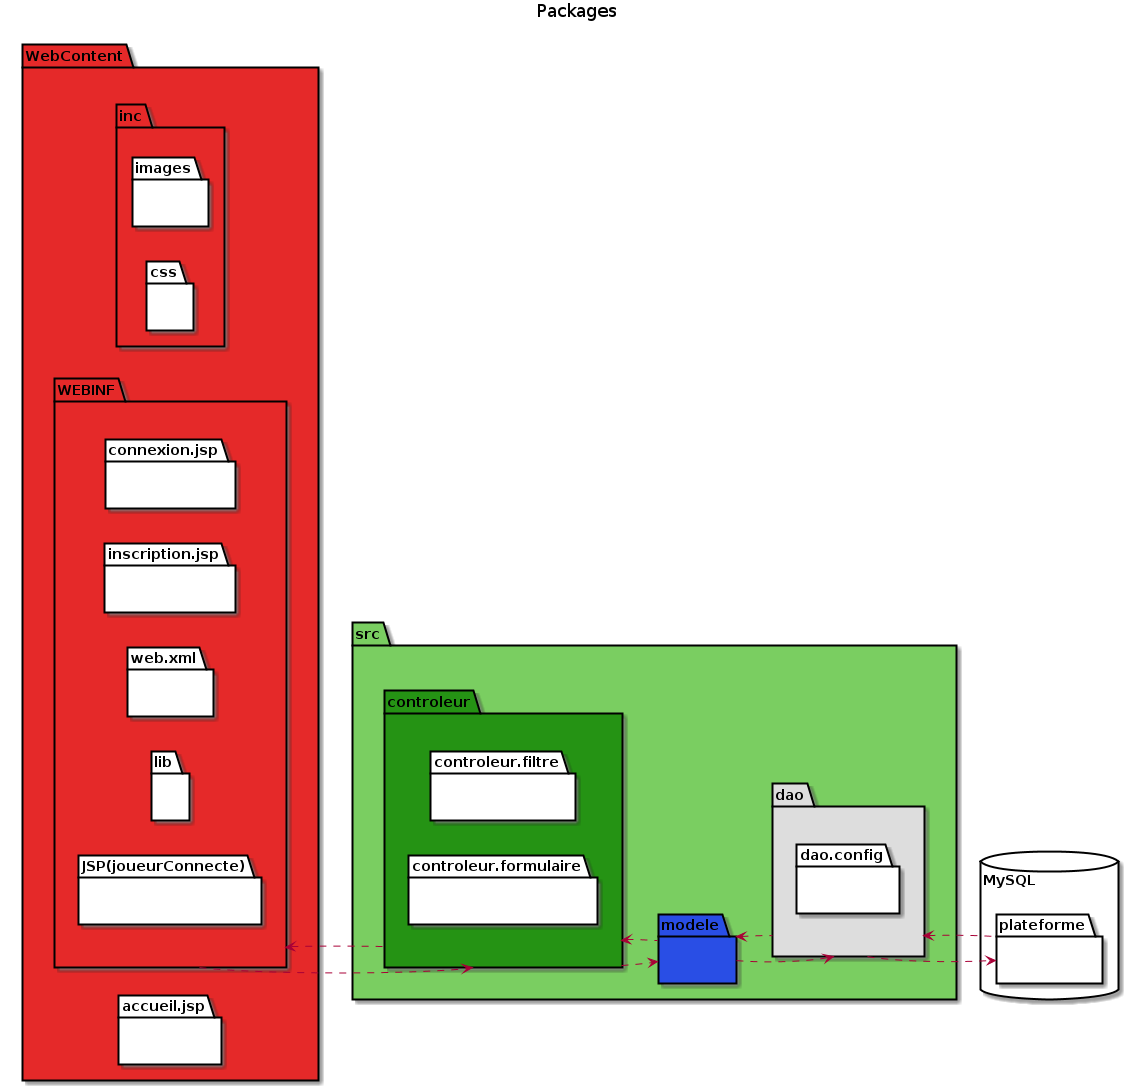
\includegraphics[scale=0.25]{../graph/packages.png} \\
  \caption{Vue d'ensemble des packages}
\end{figure}

Ce diagramme représente l'ensemble des packages qui compose notre projet. En rouge, nous retrouvons le WebContent qui correspond aux pages WEB. Le dossier inc comporte tous les fichiers qui seront inclus dans nos jsp que ce soit la feuille de style (CSS) ou bien les différentes images. Nous avons aussi la jsp qui correspond à notre page d’accueil et le package WEB-INF dans lequel se trouve toutes les autres jsp. Dans le WEB-INF nous avons également notre fichier web.xml dans lequel tous nos servlets/filtres sont définis. Ainsi que le dossier JoueurConnecte dans lequel se trouve toutes les JSP qui sont accessibles une fois que le joueur est connecte. \\

Dans le package src, nous retrouvons trois parties principales. La première correspond au controleur, il s'agit de nos servlet ainsi que du filtre qui limite l’accès à certaines pages. La partie modèle correspond au coeur de notre projet. Ce sont les classes JAVA métier de notre projet. Enfin le package DAO correspond à l'ensemble des outils nécessaires à la communication et à la modification de notre base de données. \\

Enfin la partie MySQl correspond à la partie base de données de notre programme.  

\begin{figure}[H]
  \center
  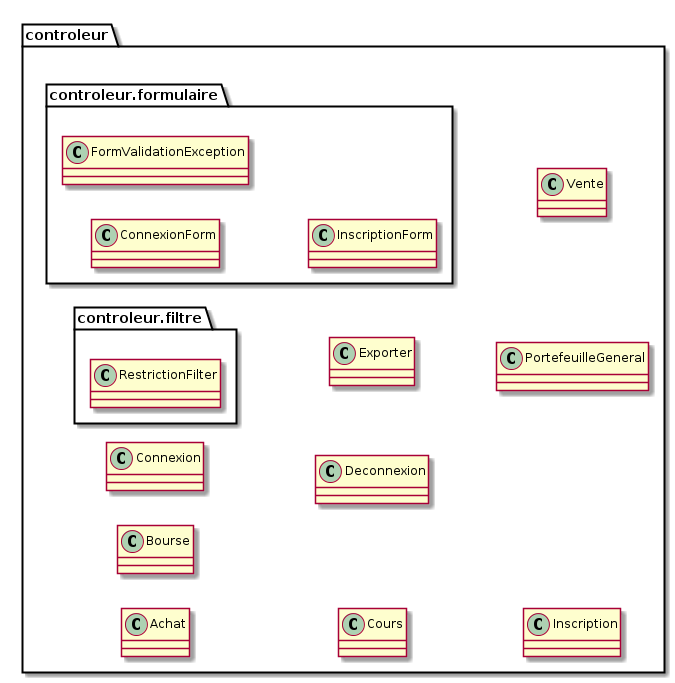
\includegraphics[scale=0.25]{../graph/packageControleur.png} \\
  \caption{Package Controleur}
\end{figure}

Ce schéma décrit plus en détail le package controleur de notre programme. On y voit en détail chacune de nos servlets qui correspondent chacune à une jsp. Par exemple, on y retrouve la servlet Achat qui va vérifier que le joueur possède assez d'argent, qu'il reste assez d'objet financier disponible pour pouvoir réaliser l'opération et enfin effectuer cette opération. Nous repérons deux packages dans le contrôleur, le premier d'entre eux correspond au filtre qui limite l'accès. Le second est un package formulaire qui permet de faire les vérifications nécessaires aux saisies effectuées par l'utilisateur lors de la connexion et de l'inscription. 
\begin{figure}[H]
  \center
  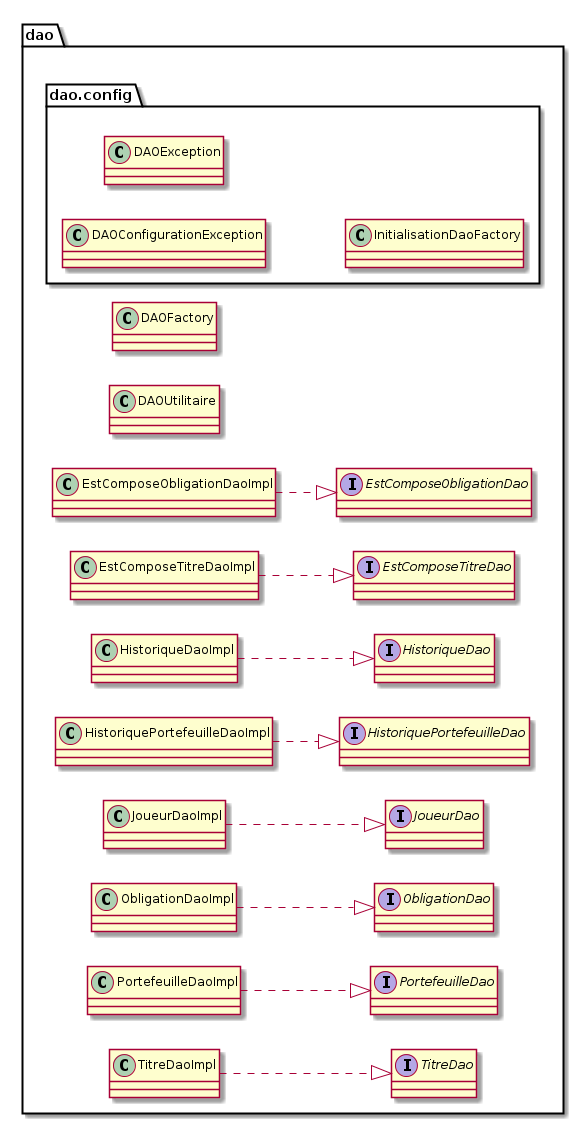
\includegraphics[scale=0.25]{../graph/packageDAO.png} \\
  \caption{package Dao}
\end{figure}

Ce diagramme décrit le package DAO. Nous voyons dans ce package un package config qui contient l'ensemble des exceptions propres à la DAO afin d'encapsuler les exceptions lors de l'exécution de requête ou lors de la configuration de l'accès à la base de données par exemple. Ensuite nous retrouvons dans ce package la DAOFactory qui permet d'instancier chacun des objet du package par exemple un JoueurDaoImpl. Ensuite la classe DAOUtilitaire permet d'avoir certaines méthodes génériques à disposition, par exemple la fermeture des différents outils utilisés, une méthode qui permet d'exécuter une requête ou de préparer une requête. Enfin, on a une interface qui définit les méthodes possibles pour effectuer des opérations avec notre table SQL, en général ce sont les opérations CRUD (Create, Read, Update et Delete). Enfin pour chacune de ces interfaces nous avons proposé une implémentation qui permet une communication avec notre table SQL pour un autre langage de base de données il faudrait proposer une nouvelle interprétation. 